% Options for packages loaded elsewhere
\PassOptionsToPackage{unicode}{hyperref}
\PassOptionsToPackage{hyphens}{url}
%
\documentclass[
]{article}
\usepackage{amsmath,amssymb}
\usepackage{iftex}
\ifPDFTeX
  \usepackage[T1]{fontenc}
  \usepackage[utf8]{inputenc}
  \usepackage{textcomp} % provide euro and other symbols
\else % if luatex or xetex
  \usepackage{unicode-math} % this also loads fontspec
  \defaultfontfeatures{Scale=MatchLowercase}
  \defaultfontfeatures[\rmfamily]{Ligatures=TeX,Scale=1}
\fi
\usepackage{lmodern}
\ifPDFTeX\else
  % xetex/luatex font selection
\fi
% Use upquote if available, for straight quotes in verbatim environments
\IfFileExists{upquote.sty}{\usepackage{upquote}}{}
\IfFileExists{microtype.sty}{% use microtype if available
  \usepackage[]{microtype}
  \UseMicrotypeSet[protrusion]{basicmath} % disable protrusion for tt fonts
}{}
\makeatletter
\@ifundefined{KOMAClassName}{% if non-KOMA class
  \IfFileExists{parskip.sty}{%
    \usepackage{parskip}
  }{% else
    \setlength{\parindent}{0pt}
    \setlength{\parskip}{6pt plus 2pt minus 1pt}}
}{% if KOMA class
  \KOMAoptions{parskip=half}}
\makeatother
\usepackage{xcolor}
\usepackage[margin=1in]{geometry}
\usepackage{color}
\usepackage{fancyvrb}
\newcommand{\VerbBar}{|}
\newcommand{\VERB}{\Verb[commandchars=\\\{\}]}
\DefineVerbatimEnvironment{Highlighting}{Verbatim}{commandchars=\\\{\}}
% Add ',fontsize=\small' for more characters per line
\usepackage{framed}
\definecolor{shadecolor}{RGB}{248,248,248}
\newenvironment{Shaded}{\begin{snugshade}}{\end{snugshade}}
\newcommand{\AlertTok}[1]{\textcolor[rgb]{0.94,0.16,0.16}{#1}}
\newcommand{\AnnotationTok}[1]{\textcolor[rgb]{0.56,0.35,0.01}{\textbf{\textit{#1}}}}
\newcommand{\AttributeTok}[1]{\textcolor[rgb]{0.13,0.29,0.53}{#1}}
\newcommand{\BaseNTok}[1]{\textcolor[rgb]{0.00,0.00,0.81}{#1}}
\newcommand{\BuiltInTok}[1]{#1}
\newcommand{\CharTok}[1]{\textcolor[rgb]{0.31,0.60,0.02}{#1}}
\newcommand{\CommentTok}[1]{\textcolor[rgb]{0.56,0.35,0.01}{\textit{#1}}}
\newcommand{\CommentVarTok}[1]{\textcolor[rgb]{0.56,0.35,0.01}{\textbf{\textit{#1}}}}
\newcommand{\ConstantTok}[1]{\textcolor[rgb]{0.56,0.35,0.01}{#1}}
\newcommand{\ControlFlowTok}[1]{\textcolor[rgb]{0.13,0.29,0.53}{\textbf{#1}}}
\newcommand{\DataTypeTok}[1]{\textcolor[rgb]{0.13,0.29,0.53}{#1}}
\newcommand{\DecValTok}[1]{\textcolor[rgb]{0.00,0.00,0.81}{#1}}
\newcommand{\DocumentationTok}[1]{\textcolor[rgb]{0.56,0.35,0.01}{\textbf{\textit{#1}}}}
\newcommand{\ErrorTok}[1]{\textcolor[rgb]{0.64,0.00,0.00}{\textbf{#1}}}
\newcommand{\ExtensionTok}[1]{#1}
\newcommand{\FloatTok}[1]{\textcolor[rgb]{0.00,0.00,0.81}{#1}}
\newcommand{\FunctionTok}[1]{\textcolor[rgb]{0.13,0.29,0.53}{\textbf{#1}}}
\newcommand{\ImportTok}[1]{#1}
\newcommand{\InformationTok}[1]{\textcolor[rgb]{0.56,0.35,0.01}{\textbf{\textit{#1}}}}
\newcommand{\KeywordTok}[1]{\textcolor[rgb]{0.13,0.29,0.53}{\textbf{#1}}}
\newcommand{\NormalTok}[1]{#1}
\newcommand{\OperatorTok}[1]{\textcolor[rgb]{0.81,0.36,0.00}{\textbf{#1}}}
\newcommand{\OtherTok}[1]{\textcolor[rgb]{0.56,0.35,0.01}{#1}}
\newcommand{\PreprocessorTok}[1]{\textcolor[rgb]{0.56,0.35,0.01}{\textit{#1}}}
\newcommand{\RegionMarkerTok}[1]{#1}
\newcommand{\SpecialCharTok}[1]{\textcolor[rgb]{0.81,0.36,0.00}{\textbf{#1}}}
\newcommand{\SpecialStringTok}[1]{\textcolor[rgb]{0.31,0.60,0.02}{#1}}
\newcommand{\StringTok}[1]{\textcolor[rgb]{0.31,0.60,0.02}{#1}}
\newcommand{\VariableTok}[1]{\textcolor[rgb]{0.00,0.00,0.00}{#1}}
\newcommand{\VerbatimStringTok}[1]{\textcolor[rgb]{0.31,0.60,0.02}{#1}}
\newcommand{\WarningTok}[1]{\textcolor[rgb]{0.56,0.35,0.01}{\textbf{\textit{#1}}}}
\usepackage{longtable,booktabs,array}
\usepackage{calc} % for calculating minipage widths
% Correct order of tables after \paragraph or \subparagraph
\usepackage{etoolbox}
\makeatletter
\patchcmd\longtable{\par}{\if@noskipsec\mbox{}\fi\par}{}{}
\makeatother
% Allow footnotes in longtable head/foot
\IfFileExists{footnotehyper.sty}{\usepackage{footnotehyper}}{\usepackage{footnote}}
\makesavenoteenv{longtable}
\usepackage{graphicx}
\makeatletter
\newsavebox\pandoc@box
\newcommand*\pandocbounded[1]{% scales image to fit in text height/width
  \sbox\pandoc@box{#1}%
  \Gscale@div\@tempa{\textheight}{\dimexpr\ht\pandoc@box+\dp\pandoc@box\relax}%
  \Gscale@div\@tempb{\linewidth}{\wd\pandoc@box}%
  \ifdim\@tempb\p@<\@tempa\p@\let\@tempa\@tempb\fi% select the smaller of both
  \ifdim\@tempa\p@<\p@\scalebox{\@tempa}{\usebox\pandoc@box}%
  \else\usebox{\pandoc@box}%
  \fi%
}
% Set default figure placement to htbp
\def\fps@figure{htbp}
\makeatother
\setlength{\emergencystretch}{3em} % prevent overfull lines
\providecommand{\tightlist}{%
  \setlength{\itemsep}{0pt}\setlength{\parskip}{0pt}}
\setcounter{secnumdepth}{-\maxdimen} % remove section numbering
\usepackage{bookmark}
\IfFileExists{xurl.sty}{\usepackage{xurl}}{} % add URL line breaks if available
\urlstyle{same}
\hypersetup{
  pdftitle={Introducción a R y Rstudio},
  hidelinks,
  pdfcreator={LaTeX via pandoc}}

\title{Introducción a R y Rstudio}
\author{}
\date{\vspace{-2.5em}2023-09-13}

\begin{document}
\maketitle

\subsection{1. Introducción}\label{introducciuxf3n}

En este taller aprenderemos a reconocer los distintos elementos en la
interfaz de RStudio, estructuras en R y manejo de datos con Tidyverse.

\subsubsection{1.1. Motivación}\label{motivaciuxf3n}

R es un lenguaje de programación y un entorno de software utilizado en
la práctica estadística y el análisis de datos. R y RStudio son
herramientas esenciales para el estudio, análisis y toma de decisiones
en salud pública, ya que permiten realizar análisis estadísticos
detallados, modelar la propagación de enfermedades, visualizar datos de
manera efectiva y automatizar tareas. Estas herramientas facilitan la
manipulación y preparación de datos, fomentan la colaboración en
proyectos de ciencia de datos, y la toma de decisiones basadas en
evidencias. Además, son útiles en la formación y educación en análisis
de datos para profesionales de la salud, áreas STEM y toma de
decisiones.

\subsubsection{1.2. Objetivos}\label{objetivos}

\begin{itemize}
\tightlist
\item
  Identificar qué son R y RStudio.
\item
  Reconocer la interfaz de RStudio.
\item
  Describir algunas estructuras básicas en R: Matrices y tablas de
  datos.
\item
  Describir el proceso de creación de funciones
\item
  Reconocer el proceso de importación, exportación y transformación de
  bases de datos con Tidyverse.
\end{itemize}

\subsubsection{1.3. Conceptos básicos a
desarrollar}\label{conceptos-buxe1sicos-a-desarrollar}

En esta práctica se desarrollarán los siguientes conceptos:

\begin{itemize}
\tightlist
\item
  Algunas estructuras básicas en R: Matrices y tablas de datos.
\item
  Importación, exportación y transformación de tablas de datos.
\end{itemize}

\subsubsection{1.4. Introducción a R}\label{introducciuxf3n-a-r}

R es un lenguaje de programación especializado para análisis de datos,
es de uso gratuito y software libre. Por otra parte, RStudio es un
editor de R también disponible de manera gratuita. En los últimos años
el uso de R ha crecido en el ámbito académico y de la industria. R,
además de ser un lenguaje de programación, es también un entorno para
computación estadística y creación de gráficos. R además de ser un
lenguaje de programación es un entorno para computación estadística y
creación de gráficos.
\href{https://cran.r-project.org/doc/html/interface98-paper/paper_2.html}{R-project}

\subsection{2. Ambiente de R}\label{ambiente-de-r}

La parte visual de RStudio está compuesta por 4 secciones principales:

\pandocbounded{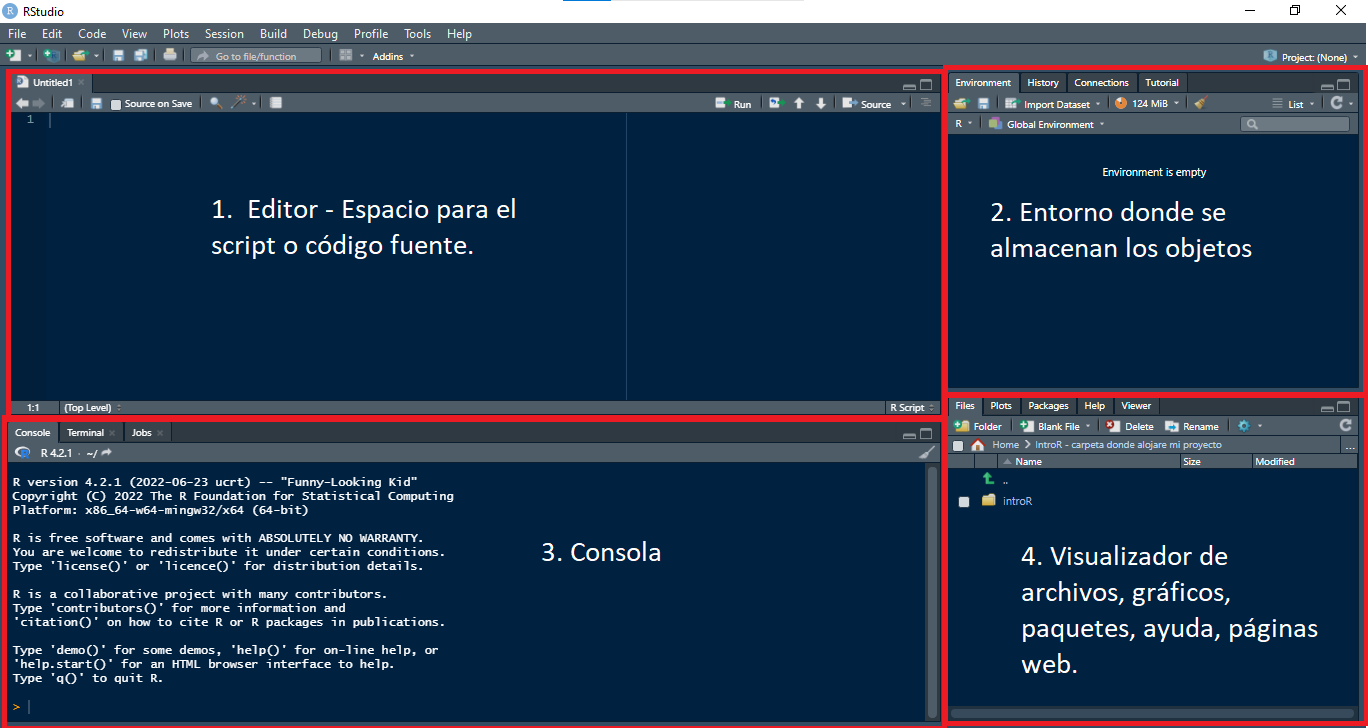
\includegraphics[keepaspectratio]{img/ambiente.png}}

\begin{enumerate}
\def\labelenumi{\arabic{enumi}.}
\item
  Editor (sección superior izquierda): esta sección es fundamental para
  la reproducibilidad del código. Este editor permite guardar el código
  para que sea usado en futuras ocasiones. El código puede ser ejecutado
  en esta sección posicionando el cursor de texto al final de la línea
  de código que se ejecutará; otra opción es seleccionando la misma y
  empleando el comando Control+Enter para Windows o Command+Enter para
  Mac.
\item
  Entorno (sección superior derecha): en esta sección se pueden
  visualizar los objetos y funciones creados o importados en la sección
  de R. Objetos como vectores, matrices, arreglos, data frames, listas,
  objetos tipo ggplot, entre otros.
\item
  Consola (sección inferior izquierda): esta sección es donde se ejecuta
  el código. No solo se ejecuta el código que escrito en el editor, sino
  que también el código puede escribirse y ejecutarse aquí directamente
  presionando Enter. Sin embargo, cuando el código se ejecuta
  directamente en la consola, este no se almacena y cuando se cierra la
  sesión de R este se pierde.
\item
  Visualizador (sección inferior derecha): en esta sección se pueden
  visualizar los archivos en ``Files'', los gráficos en ``Plots'', los
  paquetes que ya están instalados en ``Packages'', la ayuda de R con
  información de los paquetes y el funcionamiento en ``Help'', y páginas
  web en ``Viewer''.
\end{enumerate}

\subsection{3. Configuración de un proyecto en
R}\label{configuraciuxf3n-de-un-proyecto-en-r}

Una de las grandes ventajas de usar RStudio es la posibilidad de usar
los Proyectos en R (R Project)(indicado por un archivo \texttt{.Rproj})
lo que permite organizar el espacio de trabajo, el historial y los
documentos fuente.

Para crear un Proyecto en R, es importante seguir los siguientes pasos:

\begin{enumerate}
\def\labelenumi{(\arabic{enumi})}
\tightlist
\item
  Abrir RStudio y, en la esquina superior derecha, seleccionar la
  pestaña \emph{File} (Archivo) -\textgreater{} \emph{New
  Project\ldots{}} (Proyecto Nuevo).
\item
  Se desplegará una ventana con encabezado \emph{New Project Wizard:
  Create Project}, ahora se debe seleccionar \emph{New Directory}
  (Directorio Nuevo).
\end{enumerate}

\begin{figure}
\centering
\pandocbounded{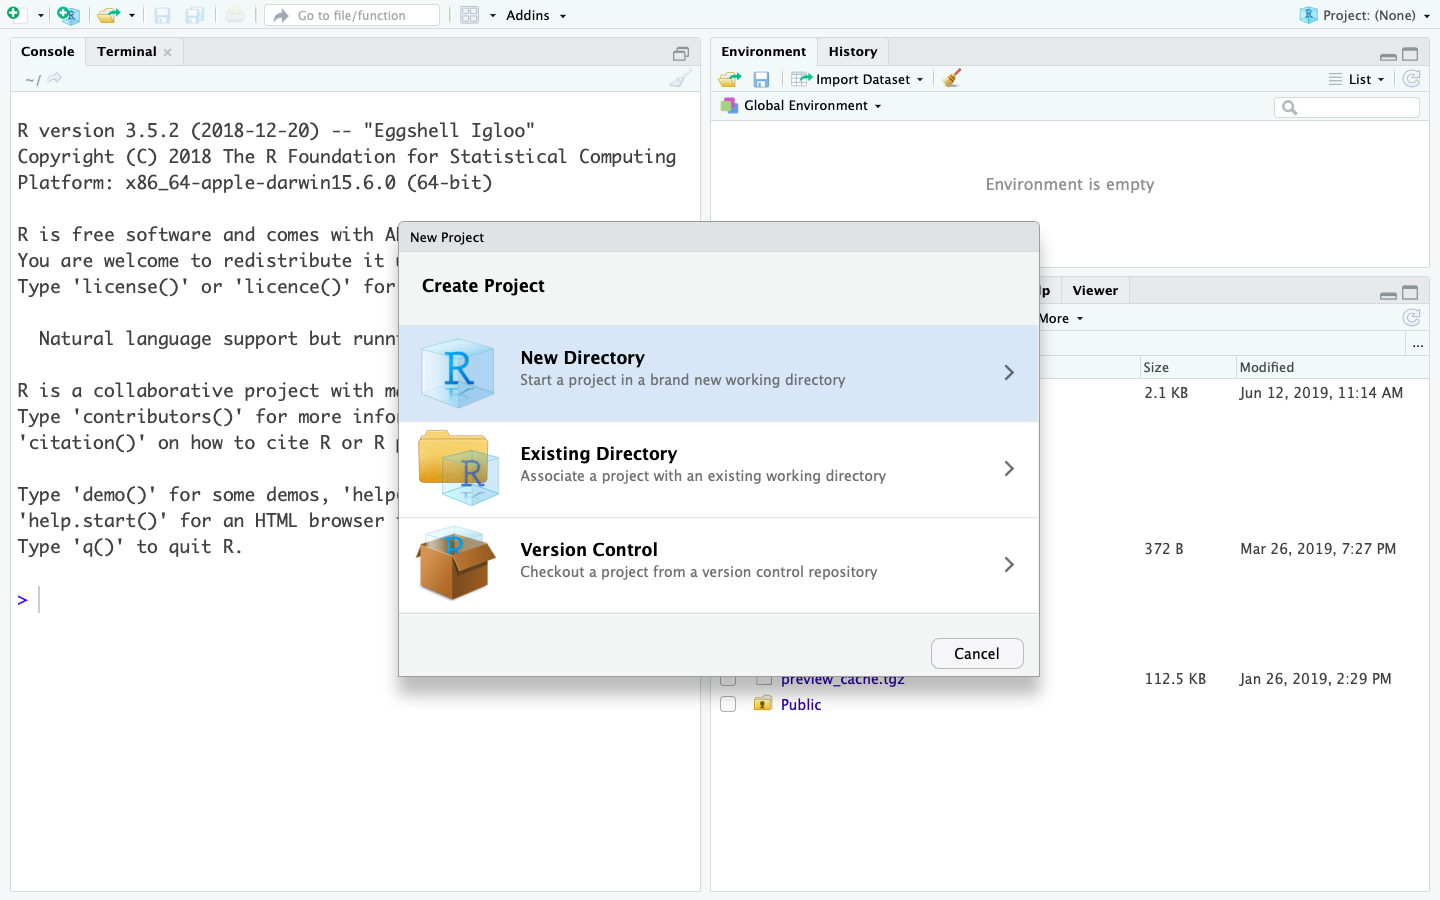
\includegraphics[keepaspectratio]{img/new_directory.png}}
\caption{Screenshot New Directory}
\end{figure}

\begin{enumerate}
\def\labelenumi{(\arabic{enumi})}
\setcounter{enumi}{2}
\item
  En la ventana \emph{Project Type}, para crear un nuevo proyecto en
  Rstudio se debe seleccionar \emph{New Project} -\textgreater{}
  \emph{Create New Project}. En la casilla \emph{Directory Name} (Nombre
  del Directorio) coloque el nombre deseado para su proyecto
  (e.g.~``introR'').
\item
  Seleccione el botón \emph{Browse\ldots{}}. En este punto, es
  conveniente crear una carpeta que servirá de repositorio para su
  proyecto, así como las sub carpetas que necesita para organizar su
  trabajo (por ejemplo: datos, scripts, figuras). Una vez creadas,
  seleccione la carpeta que servirá de repositorio.
\end{enumerate}

Al final, su proyecto debería parecerse a esta imagen

\begin{figure}
\centering
\pandocbounded{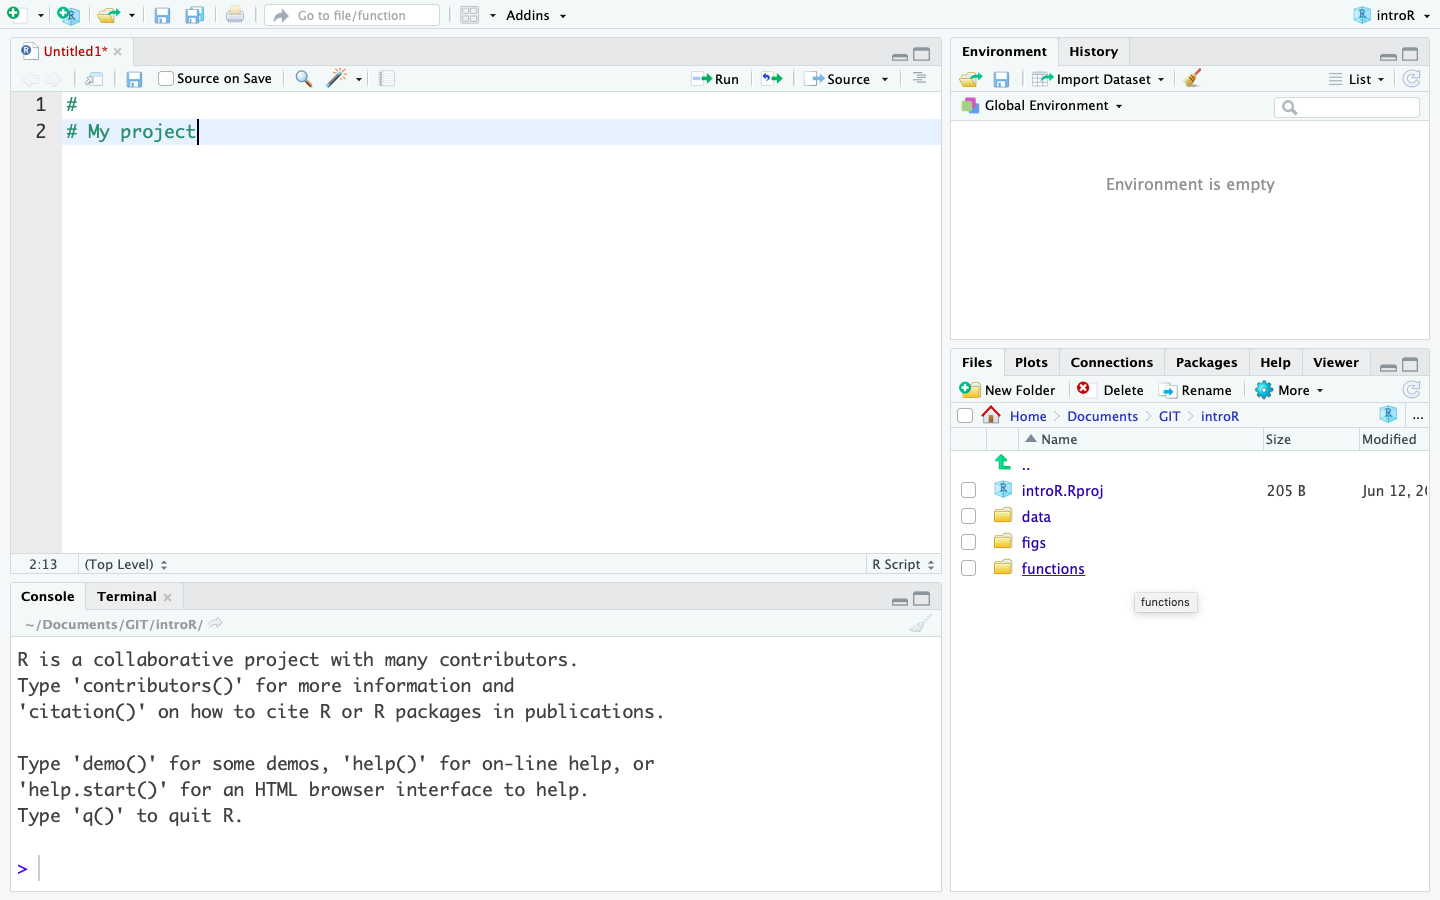
\includegraphics[keepaspectratio]{img/r_project.png}}
\caption{Screenshot R Project}
\end{figure}

\subsection{4. Estructuras en R}\label{estructuras-en-r}

\subsubsection{4.1. Vector}\label{vector}

En R, un vector es una estructura de datos indexada que permite
almacenar varios elementos del mismo tipo en una única variable. Por
ejemplo, podríamos tener un vector que contenga las edades de varias
personas, o un vector que contenga los nombres de diferentes ciudades.

Los vectores en R son útiles porque permiten realizar operaciones y
cálculos con facilidad. Los elementos del vector se pueden sumar,
restar, multiplicar o dividir, y sus elementos son accesibles por medio
posición o índice.

En resumen, un vector en R es una colección ordenada de elementos del
mismo tipo que permite almacenar y manipular datos de manera eficiente.
Es una herramienta fundamental para trabajar con datos en R y realizar
diferentes tipos de análisis y operaciones.

Los vectores se pueden crear ejecutando el comando \texttt{c()}, como se
puede visualizar a continuación:

\paragraph{Ejemplos}\label{ejemplos}

\begin{Shaded}
\begin{Highlighting}[]
\NormalTok{nombre }\OtherTok{\textless{}{-}} \FunctionTok{c}\NormalTok{(}\StringTok{"Ana"}\NormalTok{, }\StringTok{"Miguel"}\NormalTok{, }\StringTok{"Juan"}\NormalTok{, }\StringTok{"Lina"}\NormalTok{) }\CommentTok{\# Nombre de las personas}

\NormalTok{ciudad }\OtherTok{\textless{}{-}} \FunctionTok{c}\NormalTok{(}\StringTok{"Cali"}\NormalTok{,}\StringTok{"Bogota"}\NormalTok{, }\StringTok{"Medellin"}\NormalTok{, }\StringTok{"Bogota"}\NormalTok{) }\CommentTok{\# Ciudad de residencia}

\NormalTok{edad }\OtherTok{\textless{}{-}} \FunctionTok{c}\NormalTok{(}\DecValTok{15}\NormalTok{, }\DecValTok{25}\NormalTok{, }\DecValTok{32}\NormalTok{, }\DecValTok{40}\NormalTok{)  }\CommentTok{\# Edad de las personas}

\NormalTok{vacunado }\OtherTok{\textless{}{-}} \FunctionTok{c}\NormalTok{(}\ConstantTok{TRUE}\NormalTok{, }\ConstantTok{FALSE}\NormalTok{, }\ConstantTok{FALSE}\NormalTok{, }\ConstantTok{TRUE}\NormalTok{) }\CommentTok{\# Estado de vacunación}

\NormalTok{dosis }\OtherTok{\textless{}{-}} \FunctionTok{c}\NormalTok{(}\DecValTok{1}\DataTypeTok{L}\NormalTok{, }\DecValTok{0}\DataTypeTok{L}\NormalTok{, }\DecValTok{0}\DataTypeTok{L}\NormalTok{, }\DecValTok{2}\DataTypeTok{L}\NormalTok{) }\CommentTok{\# Número de dosis recibidas}
\end{Highlighting}
\end{Shaded}

\subsubsection{4.2. Data.frame (Tabla de
datos)}\label{data.frame-tabla-de-datos}

Imaginemos un Data.frame como una tabla con filas y columnas, similar a
una hoja de cálculo en Excel. Cada columna representa un tipo de
información específica o variable (Por ejemplo, la edad, el departamento
o nombre) y cada fila representa un conjunto de datos relacionados. Es
importante tener en cuenta que los Data.frame (Tabla de datos) están
compuestas por vectores cuyas dimensiones deben ser iguales, es decir
que todas las columnas deben tener el mismo número de filas.

En R, un data frame es una forma muy útil de almacenar y organizar
datos. Puede pensarse como una forma de mantener diferentes tipos de
información juntos en una estructura organizada. Por ejemplo, se puede
tener una columna para los nombres de las personas, otra para sus edades
y otra para el departamento en el que viven.

La gran ventaja de un Data.frame es que permite realizar operaciones y
análisis sobre los datos de manera ágil y eficiente. Se pueden realizar
cálculos, filtrar datos, realizar gráficos y mucho más.

En resumen, un Data.frame en R es una tabla conformada por columnas con
el mismo número de filas que permite almacenar y trabajar con diferentes
tipos de datos de manera organizada y eficiente. Por lo tanto, es una
herramienta poderosa para el análisis y manipulación de datos en R.

Para crear una tabla de datos se debe ejecutar el comando
\texttt{data.frame()}. Por ejemplo, utilizando los vectores que
definimos en la sección anterior:

\begin{Shaded}
\begin{Highlighting}[]
\NormalTok{datos\_vacunas }\OtherTok{\textless{}{-}} \FunctionTok{data.frame}\NormalTok{(}
  \AttributeTok{nombre =}\NormalTok{ nombre, }
  \AttributeTok{ciudad =}\NormalTok{ ciudad,}
  \AttributeTok{edad =}\NormalTok{ edad,}
  \AttributeTok{vacunado =}\NormalTok{ vacunado,}
  \AttributeTok{dosis =}\NormalTok{ dosis)}
\end{Highlighting}
\end{Shaded}

Tiene las siguientes propiedades:

\begin{itemize}
\tightlist
\item
  \texttt{colnames()}: nombres de las columnas
\item
  \texttt{rownames()}: nombres de las filas
\item
  \texttt{nrow()}: número de filas
\item
  \texttt{ncol()}: número de columnas
\item
  \texttt{length()}: longitud de la tabla de datos
\end{itemize}

Para acceder a la estructura general de una tabla de datos (y en general
cualquier objeto de R) usamos el comando \texttt{str}

\begin{Shaded}
\begin{Highlighting}[]
\FunctionTok{str}\NormalTok{(datos\_vacunas)}
\end{Highlighting}
\end{Shaded}

Para acceder a los diferentes componentes de la tabla de datos usamos
esta sintaxis \texttt{{[},{]}}, donde la primera dimensión corresponde a
filas y la segunda dimensión a columnas.

\begin{Shaded}
\begin{Highlighting}[]
\NormalTok{datos\_vacunas[}\DecValTok{1}\NormalTok{, }\DecValTok{2}\NormalTok{]}
\end{Highlighting}
\end{Shaded}

También es posible acceder a la información a partir de los nombres de
las columnas.

\begin{Shaded}
\begin{Highlighting}[]
\NormalTok{datos\_vacunas}\SpecialCharTok{$}\NormalTok{nombre}
\end{Highlighting}
\end{Shaded}

\paragraph{4.2.1. Importar una tabla de
datos}\label{importar-una-tabla-de-datos}

R permite a los usuarios no solo abrir, sino también crear tablas de
datos. Hay tres fuentes de conjuntos de datos:

\begin{itemize}
\tightlist
\item
  Tabla de datos importada (desde los formatos \texttt{.xlsx},
  \texttt{.csv}, \texttt{.stata}, o \texttt{.RDS}, entre otros)
\item
  Tabla de datos que forma parte de un paquete en R (Ej. MASS, islands,
  etc)
\item
  Tabla de datos creado durante la sesión en R (Ej. las estructuras de
  los primeros ejercicios)
\end{itemize}

Para importar una tabla de datos de diferentes fuentes necesitamos
emplear diferentes tipos de funciones, aquí algunos ejemplos del tipo de
datos, el paquete que es necesario cargar y la función a utilizar.

\begin{longtable}[]{@{}lll@{}}
\toprule\noalign{}
Tipo de datos & Función & Paquete \\
\midrule\noalign{}
\endhead
\bottomrule\noalign{}
\endlastfoot
csv & read\_csv & readr \\
xls & read\_excel, read\_xls,read\_xlsx & readxl \\
RDS & readRDS & base \\
dta & read\_dta & haven \\
sas & read\_sas & haven \\
sav & read\_spss & haven \\
\end{longtable}

\textbf{Abrir y explorar una tabla de datos importados de Excel}

Este es el conjunto de datos para esta práctica:
\href{https://raw.githubusercontent.com/TRACE-LAC/TRACE-LAC-data/main/datos_covid.xlsx}{datos\_covid.xlsx}:

Dentro del directorio en el que está trabajando actualmente, cree una
carpeta llamada \emph{data}. Guarde la tabla de datos descargado en la
carpeta \emph{data} que acaba de crear.

Para importar tablas de datos desde RDS, se puede usar la función
\texttt{read\_excel}, del paquete \texttt{readxl}:

\begin{Shaded}
\begin{Highlighting}[]
\FunctionTok{library}\NormalTok{(readxl)}
\NormalTok{covid19 }\OtherTok{\textless{}{-}} \FunctionTok{read\_excel}\NormalTok{(}\StringTok{"data/datos\_covid.xlsx"}\NormalTok{)}
\end{Highlighting}
\end{Shaded}

\subsection{5. Tipos de datos y operadores en
R}\label{tipos-de-datos-y-operadores-en-r}

\subsubsection{5.1. Tipos de datos}\label{tipos-de-datos}

R tiene la capacidad de almacenar y procesar distintos tipos de datos.
Entre estos se encuentran:

\begin{enumerate}
\def\labelenumi{\arabic{enumi}.}
\item
  Datos numéricos fraccionados (double. Ej: 3.3)
\item
  Datos enteros (integer. Ej: 3)
\item
  Datos en caracteres (character)
\item
  Tipos de datos booleanos/ Datos lógicos (logic. Ej: FALSE, TRUE)
\item
  Datos factor (factor. Sirven para categorizar. Ej: femenino,
  masculino, otro o primero, segundo.)
\item
  Datos tipo fechas (date. Ej: 01/01/2022)
\item
  Datos NA, NAN e Inf
\end{enumerate}

\subsubsection{5.2. Operadores}\label{operadores}

Los operadores herramientas matemáticas que nos permiten realizar
diferentes tareas con los datos que tenemos disponibles; por ejemplo,
con el operador \texttt{+} podemos efectuar una suma o incrementar un
índice. Algunos de los operadores más utilizados en R son los
siguientes:

\begin{enumerate}
\def\labelenumi{\arabic{enumi}.}
\item
  Operadores aritméticos (Ej: +, -, *)
\item
  Operadores de comparación (Ej: \textless, \textgreater, ==,
  \textgreater=, \textless=, !=)
\item
  Operadores booleanos (\& (and), \textbar{} (or), ! (not))
\end{enumerate}

\subsection{6. Funciones}\label{funciones}

Imagina una función como una especie de ``caja mágica'' que recibe
ciertos datos o información como entrada y produce un resultado o
respuesta específica como salida. Es como seguir una receta que toma
ingredientes y como resultado obtienes un plato delicioso.

Por ejemplo, considere la función \(y(x)=x+1\). Si ingresamos un dato
\(x\) (en el caso de la imagen, \(x=1\)), y aplicamos la función,
obtendremos como salida el dato \(y(1)=1+1=2\).

\begin{figure}
\centering
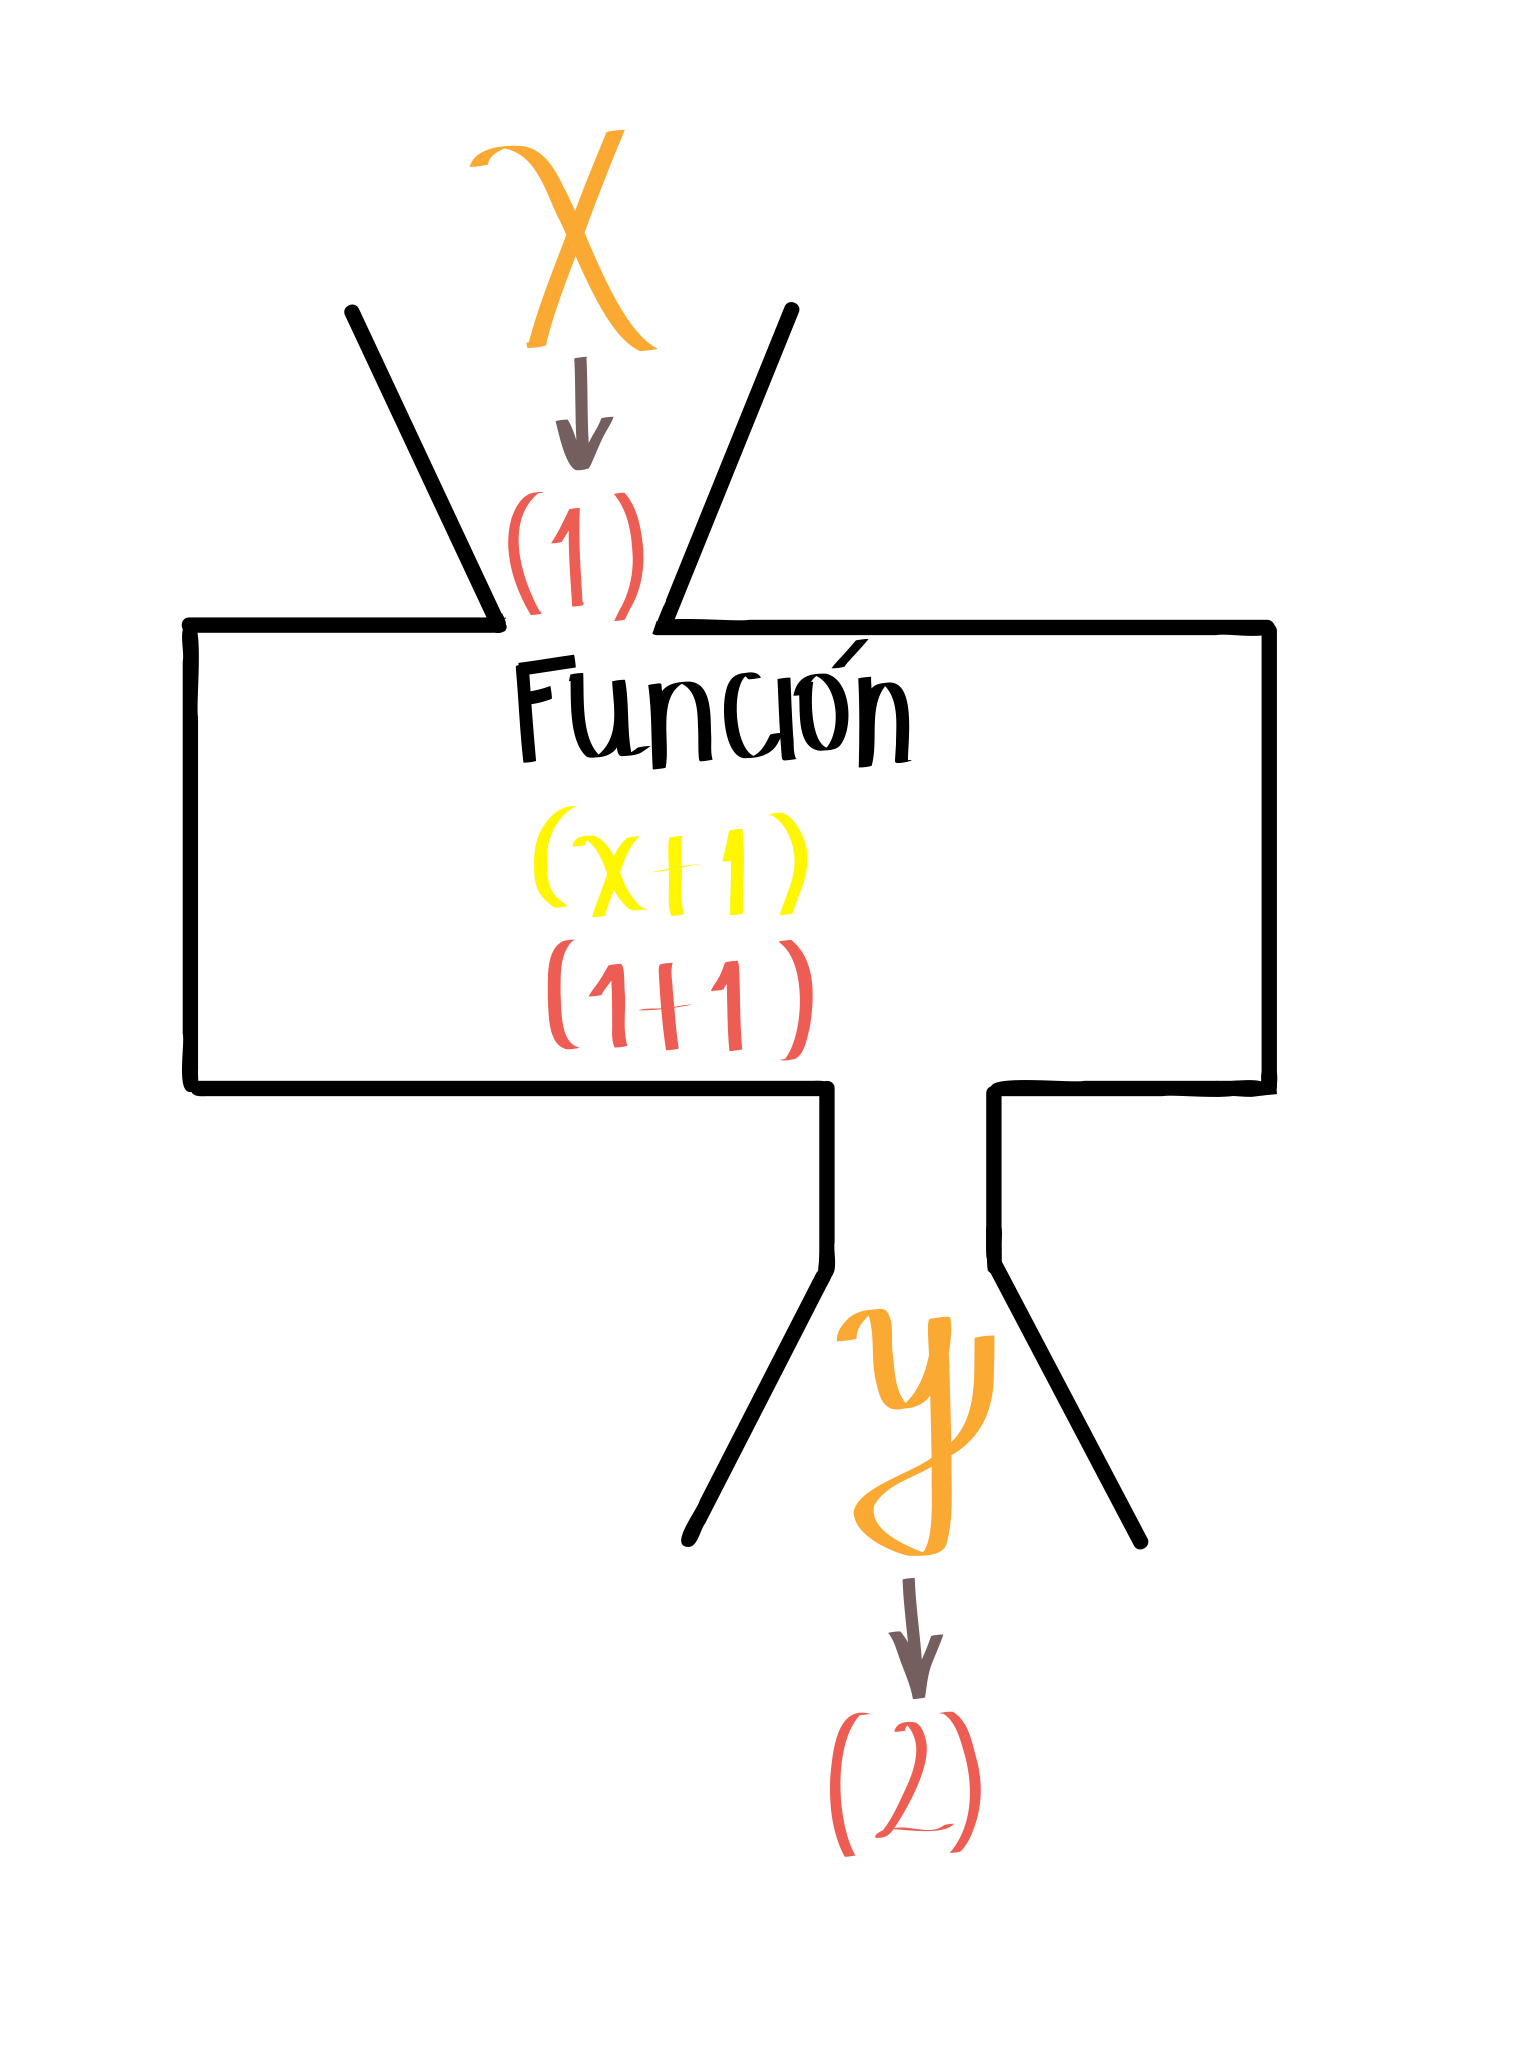
\includegraphics[width=10cm,height=\textheight,keepaspectratio]{img/ImagenFuncion.JPG}
\caption{Esquema de la función \(y(x)=x+1\).}
\end{figure}

En general, una función consiste de una secuencia de instrucciones con
el fin de llevar a cabo una tarea. De esta forma, por medio del uso de
funciones es posible sistematizar procesos complejos que se realizan de
manera rutinaria.

Los componentes básicos de una función son:

\begin{itemize}
\tightlist
\item
  \textbf{name (nombre)}: es el nombre que se da a la función(Por
  ejemplo: myfun) formals (argumentos): son la serie de elementos que
  controlan cómo llamar a la función.
\item
  \textbf{body (cuerpo):} es la serie de operaciones o modificaciones a
  los argumentos.
\item
  \textbf{output (salida o resultado)}: son los resultados después de
  modificar los argumentos. Si esta salida corresponde a una serie de
  datos, podemos extraerla usando el comando return.
\end{itemize}

\subsection{7. Manipulación de datos con
Tidyverse}\label{manipulaciuxf3n-de-datos-con-tidyverse}

Para administrar mejor los conjuntos de datos, se recomienda instalar y
utilizar el paquete \texttt{tidyverse}, el cual carga automáticamente
varios paquetes (dplyr, tidyr, tibble, readr, purr, entre otros) que son
útiles para la manipulación de datos.

\begin{Shaded}
\begin{Highlighting}[]
\FunctionTok{install.packages}\NormalTok{(}\StringTok{\textquotesingle{}tidyverse\textquotesingle{}}\NormalTok{)}
\end{Highlighting}
\end{Shaded}

\begin{Shaded}
\begin{Highlighting}[]
\FunctionTok{library}\NormalTok{(tidyverse)}
\end{Highlighting}
\end{Shaded}

A continuación, verá algunas de las funciones más utilizadas de
\texttt{tidyverse}.

\subsubsection{7.1. Operador tubería
(pipe)}\label{operador-tuberuxeda-pipe}

El operador tubería (pipe function) \texttt{\%\textgreater{}\%} es un
operador que se usa continuamente, por lo que es clave para usar
Tidyverse y facilita la programación. El operador tubería permite al
usuario enfatizar una secuencia de acciones en un objeto.

\begin{figure}
\centering
\pandocbounded{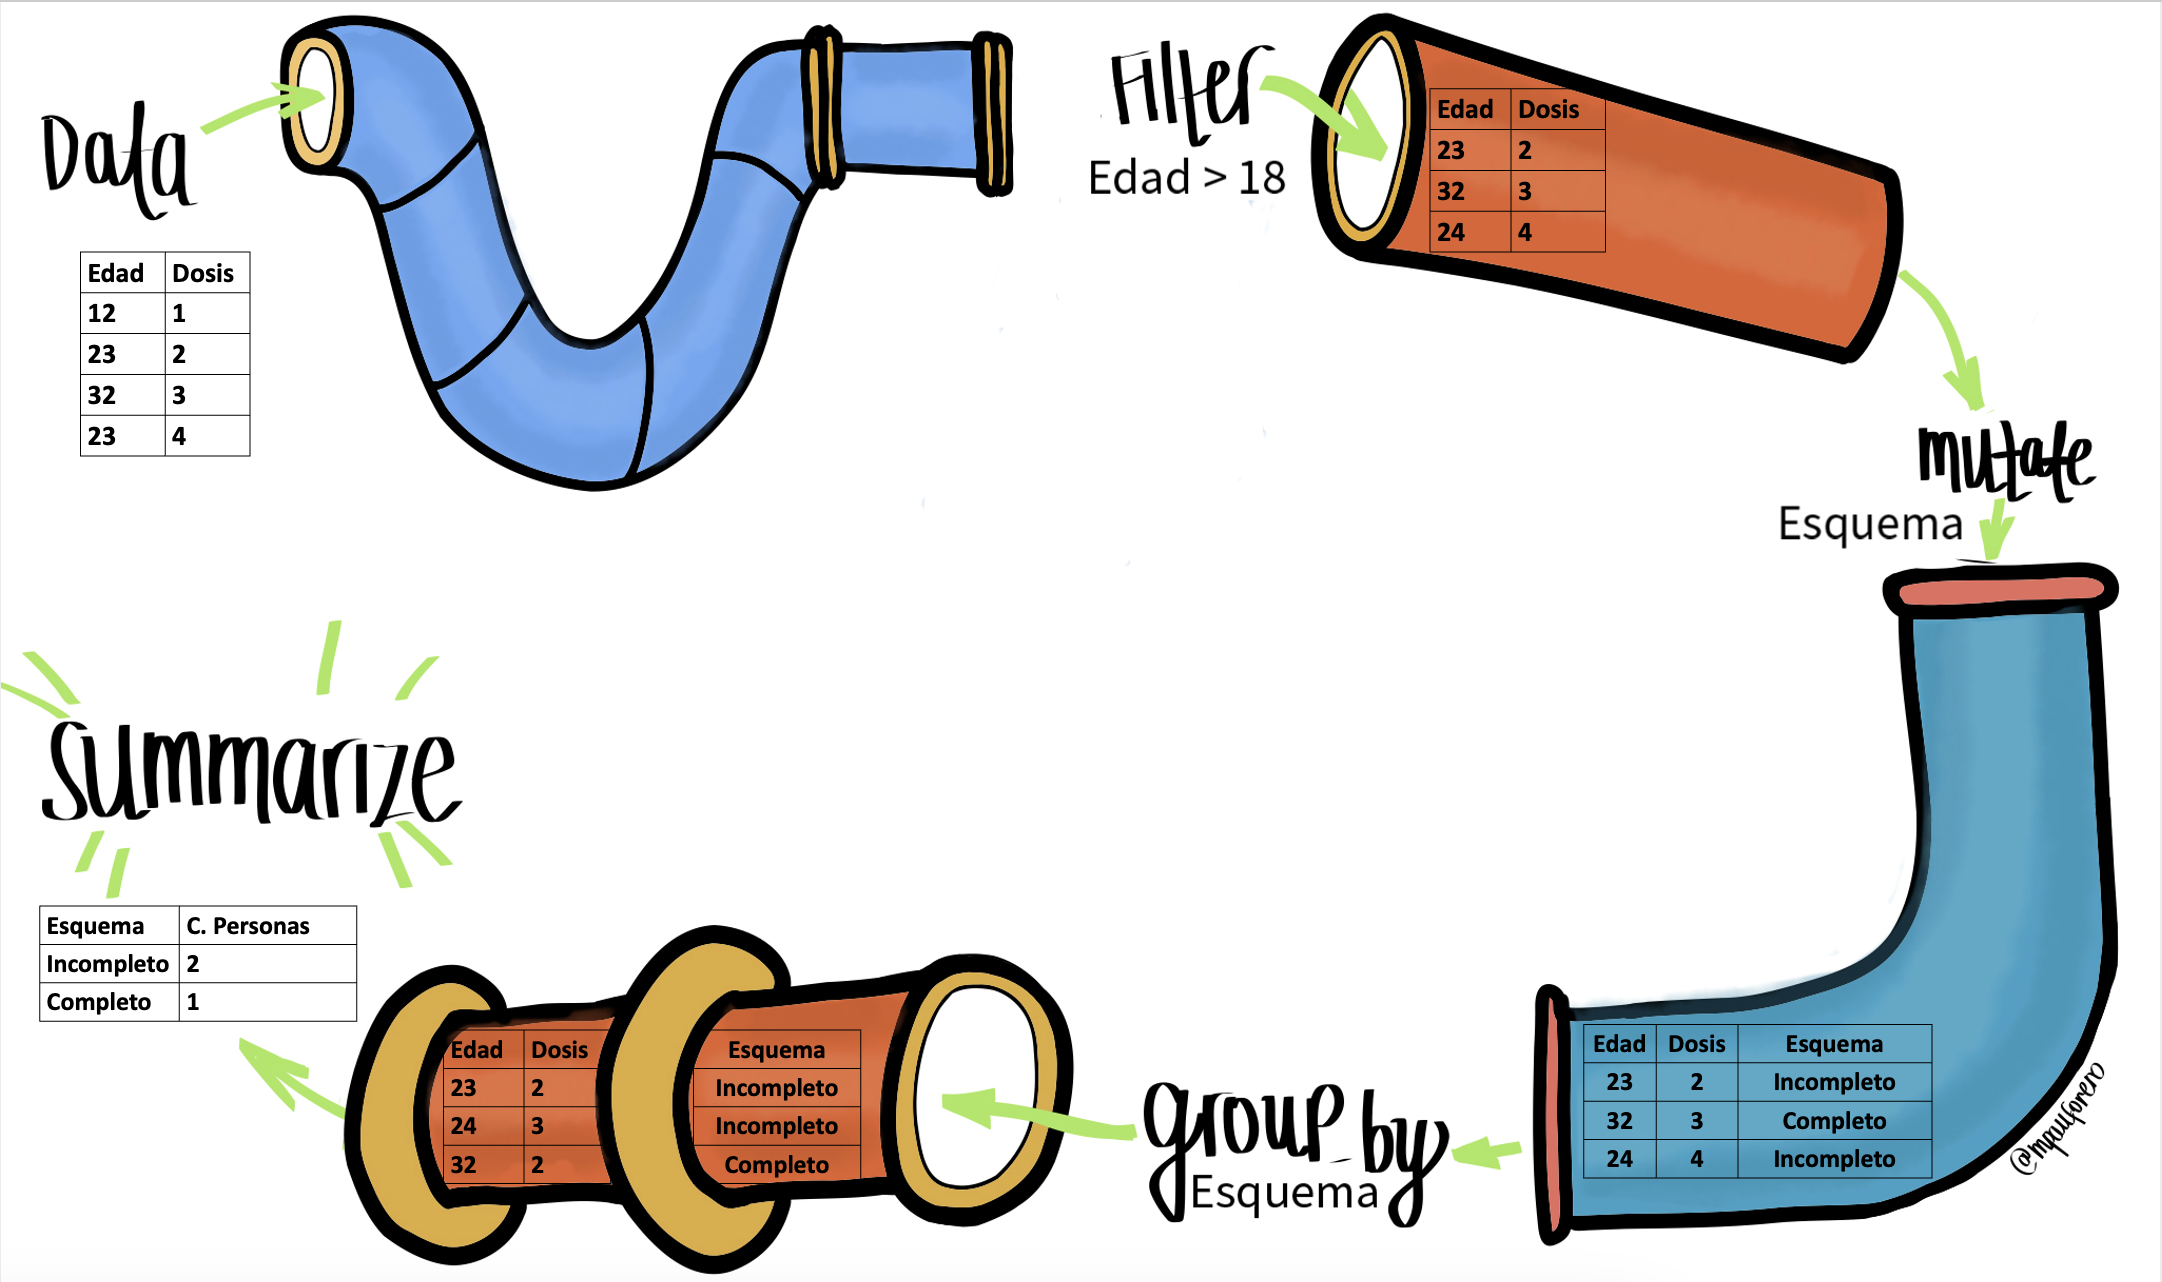
\includegraphics[keepaspectratio]{img/ImagenPipe.png}}
\caption{Esquema del operador tubería}
\end{figure}

\paragraph{Ejemplos}\label{ejemplos-1}

\textbf{Ejemplo 1}

La siguiente línea de código

\begin{Shaded}
\begin{Highlighting}[]
\FunctionTok{str}\NormalTok{(datos\_vacunas)}
\end{Highlighting}
\end{Shaded}

es equivalente a:

\begin{Shaded}
\begin{Highlighting}[]
\NormalTok{datos\_vacunas }\SpecialCharTok{\%\textgreater{}\%} \FunctionTok{str}\NormalTok{()}
\end{Highlighting}
\end{Shaded}

\textbf{Ejemplo 2} Supongamos que necesitamos sumarle 1 a una lista de
números, luego multiplicar todos sus elementos por 2 y a continuación
calcular su promedio. Sin el uso de el operador tubería, estas
operaciones se pueden realizar de la siguiente manera:

\begin{Shaded}
\begin{Highlighting}[]
\NormalTok{numeros }\OtherTok{\textless{}{-}} \FunctionTok{c}\NormalTok{(}\DecValTok{5}\NormalTok{, }\DecValTok{10}\NormalTok{, }\DecValTok{15}\NormalTok{, }\DecValTok{20}\NormalTok{)}
\NormalTok{suma\_uno }\OtherTok{\textless{}{-}}\NormalTok{ numeros }\SpecialCharTok{+} \DecValTok{1}
\NormalTok{multiplicado\_por\_dos }\OtherTok{\textless{}{-}}\NormalTok{ suma\_uno }\SpecialCharTok{*} \DecValTok{2}
\NormalTok{promedio }\OtherTok{\textless{}{-}} \FunctionTok{mean}\NormalTok{(multiplicado\_por\_dos)}
\end{Highlighting}
\end{Shaded}

Utilizando el operador tubería, la sintaxis de esta operación se puede
simplificar:

\begin{Shaded}
\begin{Highlighting}[]
\FunctionTok{library}\NormalTok{(magrittr)}
\NormalTok{numeros }\OtherTok{\textless{}{-}} \FunctionTok{c}\NormalTok{(}\DecValTok{5}\NormalTok{, }\DecValTok{10}\NormalTok{, }\DecValTok{15}\NormalTok{, }\DecValTok{20}\NormalTok{)}
\NormalTok{promedio }\OtherTok{\textless{}{-}}\NormalTok{ numeros }\SpecialCharTok{\%\textgreater{}\%}  \SpecialCharTok{+} \DecValTok{1} \SpecialCharTok{\%\textgreater{}\%} \FunctionTok{multiply\_by}\NormalTok{(}\DecValTok{2}\NormalTok{) }\SpecialCharTok{\%\textgreater{}\%}  \FunctionTok{mean}\NormalTok{()}
\end{Highlighting}
\end{Shaded}

\subsubsection{7.2. Funciones básicas de
Tidyverse}\label{funciones-buxe1sicas-de-tidyverse}

Del paquete \texttt{dyplr}, las funciones más comunes son:

\begin{itemize}
\tightlist
\item
  \texttt{glimpse}: utilizado para explorar rápidamente una tabla de
  datos
\item
  \texttt{summarise}: genera tablas resumen. Reduce las dimensiones de
  una tabla de datos
\item
  \texttt{group\_by}: crea grupos dentro de una tabla de datos. las
  funciones del \texttt{dplyr} manipulan cada grupo por separado y luego
  combina los resultados
\item
  \texttt{select}: extrae columnas de una tabla de datos
\item
  \texttt{filter}: extrae filas de una tabla de casos
\item
  \texttt{arrange}: ordena filas de una tabla de datos por el valor de
  una variable particular si es numérico, o por orden alfabético si es
  un carácter
\item
  \texttt{mutate}: genera una nueva variable
\item
  \texttt{rename}: cambia el nombre de la variable
\end{itemize}

Otra función que se utiliza continuamente en el análisis de datos es: -
\texttt{unique}: te permite extraer sólo los elementos únicos del
conjunto de datos, eliminando las repeticiones

Veamos en más detalle las funciones más comunes del paquete
\texttt{dyplr}

\subsubsection{\texorpdfstring{\texttt{glimpse}}{glimpse}}\label{glimpse}

Esta función se utiliza para explorar información de los datos como:
número de filas (que en este caso sería el número de observaciones o
datos de nuestra población), número de columnas y sus nombres (que en
este caso serían el número de variables y sus nombres), entre
``\textless{} \textgreater{}'' encontrará el tipo de dato (\texttt{dbl}
para \texttt{double}, \texttt{chr} para \texttt{character}, entre otros)
y un breve listado de algunos de los primeros valores de los datos. La
función \texttt{glimpse} se puede aplicar sobre \texttt{dat} mediante el
operador tubería como se muestra a continuación:

\begin{Shaded}
\begin{Highlighting}[]
\NormalTok{covid19 }\SpecialCharTok{\%\textgreater{}\%} \FunctionTok{glimpse}\NormalTok{()}
\end{Highlighting}
\end{Shaded}

\subsubsection{\texorpdfstring{\texttt{summarise}}{summarise}}\label{summarise}

La función \texttt{summarise} permite resumir los datos de acuerdo con
criterios definidos por funciones que retornan valores que pueden ser de
interés. Por ejemplo, para calcular la media de edad y el conteo total
de casos:

\begin{Shaded}
\begin{Highlighting}[]
\NormalTok{covid19 }\SpecialCharTok{\%\textgreater{}\%} \FunctionTok{summarise}\NormalTok{(}\AttributeTok{media =} \FunctionTok{mean}\NormalTok{(edad), }\AttributeTok{numero =} \FunctionTok{n}\NormalTok{())}
\end{Highlighting}
\end{Shaded}

\subsubsection{\texorpdfstring{\texttt{group\_by}}{group\_by}}\label{group_by}

La función \texttt{group\_by} no tiene un uso evidente si es empleada
sola, dado que ocurre un proceso interno de agrupación de los datos.
Pero al ser usada con otras funciones como por ejemplo
\texttt{summarise} es posible ver su efecto. Por ejemplo, el siguiente
comando agrupa los datos por sexo y calcula, para cada grupo, el conteo
de casos y su correspondiente media de edad:

\begin{Shaded}
\begin{Highlighting}[]
\NormalTok{covid19 }\SpecialCharTok{\%\textgreater{}\%} 
  \FunctionTok{group\_by}\NormalTok{(sexo) }\SpecialCharTok{\%\textgreater{}\%} 
  \FunctionTok{summarise}\NormalTok{(}\AttributeTok{numero =} \FunctionTok{n}\NormalTok{(), }\AttributeTok{media\_edad =} \FunctionTok{mean}\NormalTok{(edad))}
\end{Highlighting}
\end{Shaded}

\subsubsection{\texorpdfstring{\texttt{select}}{select}}\label{select}

La función \texttt{select} es útil en caso de querer extraer una o
varias columnas de un Data.frame. Por ejemplo, se puede extraer la
variable \texttt{edad} de \texttt{dat} mediante el siguiente comando:

\begin{Shaded}
\begin{Highlighting}[]
\NormalTok{covid19 }\SpecialCharTok{\%\textgreater{}\%} \FunctionTok{select}\NormalTok{(edad) }\CommentTok{\#empleando el nombre de la columna}
\NormalTok{covid19 }\SpecialCharTok{\%\textgreater{}\%} \FunctionTok{select}\NormalTok{(}\FunctionTok{c}\NormalTok{(}\DecValTok{1}\NormalTok{,}\DecValTok{2}\NormalTok{)) }\CommentTok{\#o su ubicación en los datos}
\end{Highlighting}
\end{Shaded}

\subsubsection{\texorpdfstring{\texttt{filter}}{filter}}\label{filter}

Otra función de gran utilidad es \texttt{filter}. Esta se puede usar
para seleccionar filas de acuerdo con una o más condiciones lógicas. Por
ejemplo, para filtrar los pacientes menores de 28 años:

\begin{Shaded}
\begin{Highlighting}[]
\NormalTok{covid19 }\SpecialCharTok{\%\textgreater{}\%} \FunctionTok{filter}\NormalTok{(edad }\SpecialCharTok{\textless{}} \DecValTok{28}\NormalTok{)}
\end{Highlighting}
\end{Shaded}

Como puede observar, el resultado contiene todas las variables de la
tabla, pero los datos se limitan a aquellos que en edad sean menores de
28 años.

Ahora, filtre por los pacientes de 28 años o menos de sexo femenino. En
este caso, al pedir que se incluyan adicionalmente los de 28 años
también ya no se emplea unicamente el signo ``\textless{}'' sino que se
lo acompaña del símbolo ``='':

\begin{Shaded}
\begin{Highlighting}[]
\NormalTok{covid19 }\SpecialCharTok{\%\textgreater{}\%} \FunctionTok{glimpse}\NormalTok{() }\CommentTok{\#Observe como están expresadas las variables también puede usar la función \textasciigrave{}table()\textasciigrave{}}
\NormalTok{covid19 }\SpecialCharTok{\%\textgreater{}\%} \FunctionTok{filter}\NormalTok{(sexo }\SpecialCharTok{==} \StringTok{"F"}\NormalTok{, edad }\SpecialCharTok{\textless{}=} \DecValTok{28}\NormalTok{) }\CommentTok{\#Ahora sabe como filtrar el sexo}
\end{Highlighting}
\end{Shaded}

\subsubsection{\texorpdfstring{\texttt{arrange}}{arrange}}\label{arrange}

Para los casos donde se necesita organizar los datos por una o más
variables, se puede emplear la función \texttt{arrange}. Por ejemplo,
para organizaros datos por edad, o por edad y sexo:

\begin{Shaded}
\begin{Highlighting}[]
\NormalTok{covid19 }\SpecialCharTok{\%\textgreater{}\%} \FunctionTok{arrange}\NormalTok{(edad)}
\NormalTok{covid19 }\SpecialCharTok{\%\textgreater{}\%} \FunctionTok{arrange}\NormalTok{(edad,sexo)}
\end{Highlighting}
\end{Shaded}

Por configuración predeterminada la función organiza los valores de
menor a mayor, en caso de querer organizarlos de mayor a menor se puede
emplear \texttt{desc} al interior de la función \texttt{arrange}.

\begin{Shaded}
\begin{Highlighting}[]
\NormalTok{covid19 }\SpecialCharTok{\%\textgreater{}\%} \FunctionTok{arrange}\NormalTok{(}\FunctionTok{desc}\NormalTok{(edad))}
\end{Highlighting}
\end{Shaded}

\subsubsection{\texorpdfstring{\texttt{mutate}}{mutate}}\label{mutate}

Para crear una nueva columna con datos de una ya existente resulta de
utilidad la función \texttt{mutate}. Esta función requiere el nombre de
la columna a crear y de la columna de la que queremos copiar los datos.
La columna nueva por configuración predeterminada se ubicará al final de
las variables.

\begin{Shaded}
\begin{Highlighting}[]
\FunctionTok{unique}\NormalTok{(covid19}\SpecialCharTok{$}\NormalTok{nombre\_departamento)}
\NormalTok{covid19 }\OtherTok{\textless{}{-}}\NormalTok{ covid19 }\SpecialCharTok{\%\textgreater{}\%} \FunctionTok{mutate}\NormalTok{(}\AttributeTok{nombre\_departamento =} \FunctionTok{toupper}\NormalTok{(nombre\_departamento))}
\end{Highlighting}
\end{Shaded}

\subsubsection{\texorpdfstring{\texttt{rename}}{rename}}\label{rename}

En caso de que no se desee crear una nueva variable sino renombrar una
ya existente, conviene usar la función \texttt{rename}. Por ejemplo,
cambie el nombre \emph{nombre\_departamento} por el nombre
\emph{departamento}.

\begin{Shaded}
\begin{Highlighting}[]
\NormalTok{covid19 }\SpecialCharTok{\%\textgreater{}\%} \FunctionTok{rename}\NormalTok{(}\AttributeTok{departamento =}\NormalTok{ nombre\_departamento)}
\end{Highlighting}
\end{Shaded}

\subsubsection{\texorpdfstring{\texttt{slice}}{slice}}\label{slice}

Ya se vio previamente cómo seleccionar columnas por medio de la función
\texttt{select}. En caso de requerir seleccionar filas específicas de un
Data.frame, la función \texttt{slice} resulta de gran utilidad. Por
ejemplo, para seleccionar de la fila 10 a la 15:

\begin{Shaded}
\begin{Highlighting}[]
\NormalTok{covid19 }\SpecialCharTok{\%\textgreater{}\%} \FunctionTok{slice}\NormalTok{(}\DecValTok{10}\SpecialCharTok{:}\DecValTok{15}\NormalTok{)}
\end{Highlighting}
\end{Shaded}

Alternativamente, en caso de que no se quiera emplear tidyverse, esta
acción podría realizarse mediante el siguiente comando:

\begin{Shaded}
\begin{Highlighting}[]
\NormalTok{covid19[}\DecValTok{10}\SpecialCharTok{:}\DecValTok{15}\NormalTok{, ]}
\end{Highlighting}
\end{Shaded}

Sin embargo, usar tidyverse y sus funciones resulta de gran utilidad.
Por ejemplo, suponga que necesita obtener los primeros 5 sujetos de la
base que tengan edades entre 13 y 14 años por cada sexo. Usando
tidyverse, la solución de este problema se vería así:

\begin{Shaded}
\begin{Highlighting}[]
\NormalTok{covid19 }\SpecialCharTok{\%\textgreater{}\%} 
  \FunctionTok{group\_by}\NormalTok{(sexo) }\SpecialCharTok{\%\textgreater{}\%} 
  \FunctionTok{filter}\NormalTok{(edad }\SpecialCharTok{\textgreater{}=} \DecValTok{13}\NormalTok{, edad }\SpecialCharTok{\textless{}=}\DecValTok{14}\NormalTok{) }\SpecialCharTok{\%\textgreater{}\%}
  \FunctionTok{slice}\NormalTok{(}\DecValTok{1}\SpecialCharTok{:}\DecValTok{5}\NormalTok{)}
\end{Highlighting}
\end{Shaded}

En caso de uno usar el operador tubería (pipe), el comando anterior se
vería así:

\begin{Shaded}
\begin{Highlighting}[]
\FunctionTok{slice}\NormalTok{(}\FunctionTok{filter}\NormalTok{(}\FunctionTok{group\_by}\NormalTok{(covid19, sexo),edad }\SpecialCharTok{\textgreater{}=} \DecValTok{13}\NormalTok{, edad }\SpecialCharTok{\textless{}=}\DecValTok{14}\NormalTok{),}\DecValTok{1}\SpecialCharTok{:}\DecValTok{5}\NormalTok{)}
\end{Highlighting}
\end{Shaded}

Como puede notar, el resultado es idéntico. Sin embargo, es preferible
usar el operador tubería cuando se aplican varias funciones
sucesivamente sobre un objeto porque simplifica la sintaxis del código
y, como se puede ver, la lectura del mismo se hace más sencilla. Además,
emplear el operador tubería facilita la modificación del proceso en caso
de ser necesario.

\subsection{8. Reto}\label{reto}

Esta vez se cargará un tipo diferente de datos, estos los puede
encontrar en el enlace
\url{https://github.com/TRACE-LAC/TRACE-LAC-data/blob/main/datos_covid.RDS?raw=true}.
Los datos pueden ser cargados desde el computador o desde una ubicación
en internet. Para este ejercicio cargue la base de datos
datos\_covid.RDS directamente desde internet con los comandos:

\begin{Shaded}
\begin{Highlighting}[]
\NormalTok{url }\OtherTok{\textless{}{-}} \StringTok{"https://github.com/TRACE{-}LAC/TRACE{-}LAC{-}data/blob/main/datos\_covid.RDS?raw=true"}

\NormalTok{covid19 }\OtherTok{\textless{}{-}}\NormalTok{ readr}\SpecialCharTok{::}\FunctionTok{read\_rds}\NormalTok{(url)}
\end{Highlighting}
\end{Shaded}

Por favor, realice las siguientes actividades:

\begin{itemize}
\tightlist
\item
  \textbf{Explore los datos}
\end{itemize}

Como puede observar los nombres de las columnas (variables) están con
algunas letras en mayúsculas, otras con tildes y con espacios. Lo
primero que es necesario hacer es poner los nombres en una forma que
permitan evitar errores, es decir, todos en minúsculas, sin caracteres
especiales, tildes ni espacios. Para ello se usará la función
\texttt{clean\_labels} del paquete \texttt{epitrix}.

\begin{Shaded}
\begin{Highlighting}[]
\CommentTok{\#Primero se llamarán los nombres de las variables con la función \textasciigrave{}names\textasciigrave{}}
\FunctionTok{names}\NormalTok{(covid19)}
\CommentTok{\#ahora a estos nombres se les reasignará nombres limpios}
\FunctionTok{names}\NormalTok{(covid19) }\OtherTok{\textless{}{-}} \FunctionTok{names}\NormalTok{(covid19) }\SpecialCharTok{\%\textgreater{}\%}\NormalTok{ epitrix}\SpecialCharTok{::}\FunctionTok{clean\_labels}\NormalTok{()}

\FunctionTok{names}\NormalTok{(covid19)}
\end{Highlighting}
\end{Shaded}

Ahora que los nombres están limpios es posible seguir.

\begin{itemize}
\tightlist
\item
  Filtre los datos para Cali (observe bien cómo están escritos los datos
  dentro de la variables)
\item
  Agrupe los datos por departamento y cuente los casos por cada uno.
\item
  Agrupe los datos por departamento y saque la media de edad de cada
  uno.
\item
  Cambie el nombre de estado por gravedad.
\item
  Ordene los datos por sexo y seleccione las 5 primeras filas de cada
  uno.
\item
  Haga una tabla que muestre cuantas personas de cada etnia aparecen en
  la base ubicados en la ciudad de Bogota.
\item
  Seleccione las 5 primeras filas de solo el número de identificación
  del caso.
\end{itemize}

\subsubsection{Enlaces utiles}\label{enlaces-utiles}

\href{http://people.umass.edu/biep640w/pdf/RStudio101\%20-\%20Introduction\%20by\%20Oscar\%20Torres-Reyna.pdf}{Introducción
a R}

\href{https://www.genbeta.com/desarrollo/introduccion-a-r-historia-de-un-lenguaje-de-computacion-para-el-analisis-de-datos}{Historia
de R}

\subsection{Contribuciones}\label{contribuciones}

\begin{itemize}
\tightlist
\item
  Zulma M. Cucunuba: Versión inicial
\item
  Zhian N. Kamvar: Ediciones menores
\item
  Kelly A. Charniga: Ediciones menores
\item
  José M. Velasco-España: Traducción de Inglés a Español y edición
\item
  Andree Valle-Campos: Ediciones menores
\item
  Miguel E. Gámez López: Ediciones menores
\item
  Nicolás T. Domínguez: Ediciones menores
\item
  Jaime A. Pavlich-Mariscal: Edición
\end{itemize}

Contribuciones son bienvenidas vía
\href{https://github.com/reconhub/learn/pulls}{pull requests}.

\subsection{Asuntos legales}\label{asuntos-legales}

\textbf{Licencia}:
\href{https://creativecommons.org/licenses/by/3.0/}{CC-BY}
\textbf{Copyright}: Zulma M. Cucunuba, 2019

\end{document}
